% Chapter Template

\chapter{XMLSignature} % Main chapter title

\label{Chapter: XMLSignature} % Change X to a consecutive number; for referencing this chapter elsewhere, use \ref{ChapterX}

\lhead{Chapter 6. \emph{XMLSignature}} % Change X to a consecutive number; this is for the header on each page - perhaps a shortened title

%----------------------------------------------------------------------------------------
%       SECTION 1
%----------------------------------------------------------------------------------------

\section{Introduction}
Although privacy is a solved question with XMLEncryption, there are other aspects of the security that XMLEncryption can't cover. For example:

\begin{itemize}
\item We want nobody to modify parts of a Petri net
\item I want to put on record that I am the author or the responsive of a
Petri net
\item Maybe I want to be sure that the author of a Petri net is somebody
with no doubt
\end{itemize}

To solve these questions, we can use digital signature. It gives us several
interenting characteristics:
\begin{itemize}
\item \textbf{Integrity}: The data integrity will appear if we are able to
avoid, or at least detect, any non authorized modification of the information
\item \textbf{Authentication}: authentication guarantee that somebody is
who says that he is. Basically, with digital signature nobody can impersonate another.
\item \textbf{Non repudiation}: with this characteristic, we can avoid that
somebody says he hasn't signed something if he really did. Only that person
can have done it.

\end{itemize}

In this case I want to sign a whole Petri net or concrete parts of it. Obviously,
if I sign only of a Petri net, this part keeps integrity, authentication
and non repudiation, but the rest of it doesn't.

As with XMLEncryption, the best way to achieve this goals is using standard
technologies. For signing, the method chosen is XMLSignature \cite{XMLSIG-w3.org/xmlsig-core1}.


\section{XMLSignature revision}
XMLSignature is a digital signing standard. With XMLSignature we can sign any kind of content but the result is XML content. It requires the use of
digital certificates and a set of public/private keys, using asymmetrical
ciphering algorithms for the process.

It has three possibilities:

\begin{enumerate}
\item \textbf{Enveloped}: The result of the signing is the original xml file
with a new attached signature element inside.
\item \textbf{Enveloping}: The result of the signing is a new xml file with
the digital signature, and, inside it, the original signed elements of the initial xml file.
\item \textbf{Detached}: The result of the signature is a new independent file.
The original xml file remains inalterable, The new file contains the sign.
\end{enumerate}

It is indifferent which of this three methods use. They are only different
ways to organize the generated signature. 

XMLSignature forces a digital signature to have:
\begin{itemize}
\item \textbf{Canonicalization method}: Basically, we have an equivalent relationship
that is able to detect if two xml files are equivalent each other. A canonicalization method transforms a xml file into a canonicalized one that is the representant
of the equivalence class. All the equivalent xml files are transformed
in this representant. This transform has to be applied before signing. If no method is declared, there is one defined by default.
\item \textbf{Reference}: there can be several references in one only signature.
Each reference indicates a part of the document that has to be signed and
the digest algorithm used. \footnote{A digest algorithm generates a fixed length
bytes sequence from arbitrary length contents. This bytes sequence is different
for each content}. It is important to say that each reference doesn't generate
a signature, but all of these references are signed together and generates only
one signature.
\item \textbf{Key information}: Optionally, the signature can include necessary
information to be validated. In this part we can indicate the public key
directly, by a bytes sequence, by an URL or the most usual X.509 digital certificates.\item \textbf{Transforms}: It is possible that that we want to sign is not
the whole document, but concrete information obtained from it (but not the
content itself): e.g. encoding/decoding, select only certain parts, modify the XML structure,
include fragments of other documents,... Transforms is a ordered list of
processing steps that has to be applied to the content before being digested.  This feature is optional but in this case it will be necessary.
\end{itemize}

A XML signature consists of a \texttt{<Signature>}
tag defined in the \texttt{http://www.w3.org/2000/09/xmldsig\#}# namespace.

The basic structure of the element signature is:

\begin{lstlisting}
<Signature>
  <SignedInfo>
    <CanonicalizationMethod />
    <SignatureMethod />
    <Reference>
      <Transforms>
        <Transform />
      </Transforms> 
      <DigestMethod>
      <DigestValue>
    </Reference>
    <Reference /> etc.
  </SignedInfo>
  <SignatureValue />
  <KeyInfo />
  <Object />
</Signature>
\end{lstlisting}

The element \texttt{<Object>} is used only in enveloping signature to store
the signed data. In this case I am going to use enveloped signature, so this
element will no be present in the examples.

The final aspect of a complete XMLSignature element is like this example:

\begin{lstlisting}
<Signature xmlns="http://www.w3.org/2000/09/xmldsig#">  
  <SignedInfo xmlns="http://www.w3.org/2000/09/xmldsig#">  
    <CanonicalizationMethod  
        Algorithm="http://www.w3.org/TR/2001/REC-xml-c14n-20010315"  
        xmlns="http://www.w3.org/2000/09/xmldsig#" />  
    <SignatureMethod  
        Algorithm="http://www.w3.org/2000/09/xmldsig#dsa-sha1"  
        xmlns="http://www.w3.org/2000/09/xmldsig#" />  
    <Reference URI=""  
        xmlns="http://www.w3.org/2000/09/xmldsig#">  
      <Transforms  
          xmlns="http://www.w3.org/2000/09/xmldsig#">  
        <Transform  
            Algorithm="http://www.w3.org/2000/09/xmldsig#enveloped-signature"
            xmlns="http://www.w3.org/2000/09/xmldsig#" />  
      </Transforms>  
      <DigestMethod  
          Algorithm="http://www.w3.org/2000/09/xmldsig#sha1"  
          xmlns="http://www.w3.org/2000/09/xmldsig#" />  
      <DigestValue
          xmlns="http://www.w3.org/2000/09/xmldsig#">  
        Oyyx+K28+cp7kuUgcnANtTBdUwg=  
      </DigestValue>
    </Reference>  
  </SignedInfo>  
  <SignatureValue xmlns="http://www.w3.org/2000/09/xmldsig#">  
    ZVzRud7G4mEZsDnBavbnZoFUmm5J2OBDkQ+IooDLn95ndGYdrq6uPQ==  
  </SignatureValue>  
  <KeyInfo xmlns="http://www.w3.org/2000/09/xmldsig#">  
    <X509Data xmlns="http://www.w3.org/2000/09/xmldsig#">  
      <X509Certificate  
          xmlns="http://www.w3.org/2000/09/xmldsig#">  
        IICmDCCAlYCBEfrim8wCwYHKoZIzjgEAwUAMDIxCzAJBgNVBAYTAkVTMREwDwYDVQQKEwhBd
        pYTEQMA4GA1UEAxMHVXN1YXJpbzAeFw0wODAzMjcxMTUyMTVaFw0wOTAzMjcxMTUyMTVaMDI
        BgNVBAYTAkVTMREwDwYDVQQKEwhBdXRlbnRpYTEQMA4GA1UEAxMHVXN1YXJpbzCCAbcwggEs
        BgcqhkjOOAQBMIIBHwKBgQD9f1OBHXUSKVLfSpwu7OTn9hG3UjzvRADDHj+AtlEmaUVdQCJR
        jVj6v8X1ujD2y5tVbNeBO4AdNG/yZmC3a5lQpaSfn+gEexAiwk+7qdf+t8Yb+DtX58aophUP
        9tPFHsMCNVQTWhaRMvZ1864rYdcq7/IiAxmd0UgBxwIVAJdgUI8VIwvMspK5gqLrhAvwWBz1
        APfhoIXWmz3ey7yrXDa4V7l5lK+7+jrqgvlXTAs9B4JnUVlXjrrUWU/mcQcQgYC0SRZxI+hM
        t88JMozIpuE8FnqLVHyNKOCjrh4rs6Z1kW6jfwv6ITVi8ftiegEkO8yk8b6oUZCJqIPf4Vrl
        i2ZegHtVJWQBTDv+z0kqA4GEAAKBgDUPDwxDZFXMrZha74VNmgyFslLM01wKw17nbt9UFTJA
        iPpozeZMP2u0SoYst2nbxkCs1hziiuaNJnykzcjVf3+PmL3sQES8SxwJBRUME2UTA2006WD3
        iZ9yibcWQimB8eKIJyBBxSk5TueAzvTA8HN2+Rvgh8RMaOzhMAsGByqGSM44BAMFAAMvADAs
        4+nQZdFvlvsfyOfq1t02h9MJEgIUEvYDfxeygKCmrIlA0sQLtaCs0Qo=
      </X509Certificate>  
    </X509Data>  
    <KeyValue xmlns="http://www.w3.org/2000/09/xmldsig#">  
      <DSAKeyValue  
          xmlns="http://www.w3.org/2000/09/xmldsig#">  
        <P xmlns="http://www.w3.org/2000/09/xmldsig#">  
          /X9TgR11EilS30qcLuzk5/YRt1I870QAwx4/gLZRJmlFXUAiUftZPY1Y+r/F9bow9subVWz
          HTRv8mZgt2uZUKWkn5/oBHsQIsJPu6nX/rfGG/g7V+fGqKYVDwT7g/bTxR7DAjVUE1oWkTL
          K2HXKu/yIgMZndFIAcc=  
        </P>  
        <Q xmlns="http://www.w3.org/2000/09/xmldsig#">  
          l2BQjxUjC8yykrmCouuEC/BYHPU=  
        </Q>  
        <G xmlns="http://www.w3.org/2000/09/xmldsig#">  
          9+GghdabPd7LvKtcNrhXuXmUr7v6OuqC+VdMCz0HgmdRWVeOutRZT+ZxBxCBgLRJFnEj6Ew
          zwkyjMim4TwWeotUfI0o4KOuHiuzpnWRbqN/C/ohNWLx+2J6ASQ7zKTxvqhRkImog9/hWuW
          Zl6Ae1UlZAFMO/7PSSo=  
        </G>  
        <Y xmlns="http://www.w3.org/2000/09/xmldsig#">  
          NQ8PDENkVcytmFrvhU2aDIWyUszTXArDXudu31QVMkAuTvWI+mjN5kw/a7RKhiy3advGQKz
          5o0mfKTNyNV/f4+YvexARLxLHAkFFQwTZRMDbTTpYPfE3L2Jn3KJtxZCKYHx4ognIEHFKTl
          9MDwc3b5G+CHxExo7OE=  
        </Y>  
      </DSAKeyValue>  
    </KeyValue>  
  </KeyInfo>  
</Signature>
\end{lstlisting}

At first sight it seems very complicated, but it isn't.
First of all, the attribute xmlns that is in almost all the tags is only
the namespace. From here, for more clarity it can be obviated. So the example
is as follows:
\begin{lstlisting}
<Signature>  
  <SignedInfo>  
    <CanonicalizationMethod 
        Algorithm="http://www.w3.org/TR/2001/REC-xml-c14n-20010315" />  
    <SignatureMethod  
        Algorithm="http://www.w3.org/2000/09/xmldsig#dsa-sha1" />  
    <Reference URI="">  
      <Transforms>  
        <Transform  
            Algorithm="http://www.w3.org/2000/09/xmldsig#enveloped-signature"/>
      </Transforms>  
      <DigestMethod  
          Algorithm="http://www.w3.org/2000/09/xmldsig#sha1" />  
      <DigestValue>  
        Oyyx+K28+cp7kuUgcnANtTBdUwg=  
      </DigestValue>
    </Reference>  
  </SignedInfo>  
  <SignatureValue>  
    ZVzRud7G4mEZsDnBavbnZoFUmm5J2OBDkQ+IooDLn95ndGYdrq6uPQ==  
  </SignatureValue>  
  <KeyInfo>  
    <X509Data>  
      <X509Certificate>  
        IICmDCCAlYCBEfrim8wCwYHKoZIzjgEAwUAMDIxCzAJBgNVBAYTAkVTMREwDwYDVQQKEwhBd
        pYTEQMA4GA1UEAxMHVXN1YXJpbzAeFw0wODAzMjcxMTUyMTVaFw0wOTAzMjcxMTUyMTVaMDI
        BgNVBAYTAkVTMREwDwYDVQQKEwhBdXRlbnRpYTEQMA4GA1UEAxMHVXN1YXJpbzCCAbcwggEs
        BgcqhkjOOAQBMIIBHwKBgQD9f1OBHXUSKVLfSpwu7OTn9hG3UjzvRADDHj+AtlEmaUVdQCJR
        jVj6v8X1ujD2y5tVbNeBO4AdNG/yZmC3a5lQpaSfn+gEexAiwk+7qdf+t8Yb+DtX58aophUP
        9tPFHsMCNVQTWhaRMvZ1864rYdcq7/IiAxmd0UgBxwIVAJdgUI8VIwvMspK5gqLrhAvwWBz1
        APfhoIXWmz3ey7yrXDa4V7l5lK+7+jrqgvlXTAs9B4JnUVlXjrrUWU/mcQcQgYC0SRZxI+hM
        t88JMozIpuE8FnqLVHyNKOCjrh4rs6Z1kW6jfwv6ITVi8ftiegEkO8yk8b6oUZCJqIPf4Vrl
        i2ZegHtVJWQBTDv+z0kqA4GEAAKBgDUPDwxDZFXMrZha74VNmgyFslLM01wKw17nbt9UFTJA
        iPpozeZMP2u0SoYst2nbxkCs1hziiuaNJnykzcjVf3+PmL3sQES8SxwJBRUME2UTA2006WD3
        iZ9yibcWQimB8eKIJyBBxSk5TueAzvTA8HN2+Rvgh8RMaOzhMAsGByqGSM44BAMFAAMvADAs
        4+nQZdFvlvsfyOfq1t02h9MJEgIUEvYDfxeygKCmrIlA0sQLtaCs0Qo=
      </X509Certificate>  
    </X509Data>  
    <KeyValue>  
      <DSAKeyValue>  
        <P>  
          /X9TgR11EilS30qcLuzk5/YRt1I870QAwx4/gLZRJmlFXUAiUftZPY1Y+r/F9bow9subVWz
          HTRv8mZgt2uZUKWkn5/oBHsQIsJPu6nX/rfGG/g7V+fGqKYVDwT7g/bTxR7DAjVUE1oWkTL
          K2HXKu/yIgMZndFIAcc=  
        </P>  
        <Q>  
          l2BQjxUjC8yykrmCouuEC/BYHPU=  
        </Q>  
        <G>  
          9+GghdabPd7LvKtcNrhXuXmUr7v6OuqC+VdMCz0HgmdRWVeOutRZT+ZxBxCBgLRJFnEj6Ew
          zwkyjMim4TwWeotUfI0o4KOuHiuzpnWRbqN/C/ohNWLx+2J6ASQ7zKTxvqhRkImog9/hWuW
          Zl6Ae1UlZAFMO/7PSSo=  
        </G>  
        <Y>  
          NQ8PDENkVcytmFrvhU2aDIWyUszTXArDXudu31QVMkAuTvWI+mjN5kw/a7RKhiy3advGQKz
          5o0mfKTNyNV/f4+YvexARLxLHAkFFQwTZRMDbTTpYPfE3L2Jn3KJtxZCKYHx4ognIEHFKTl
          9MDwc3b5G+CHxExo7OE=  
        </Y>  
      </DSAKeyValue>  
    </KeyValue>  
  </KeyInfo>  
</Signature>
\end{lstlisting}

 

\section{XMLSignature and Petri nets}

In this case I am going to use enveloped signature, so the result of the
signature is a stored in a new tag inside the original PNML file.
As I explained before, we have to select which parts of the PNML file are
going to be signed.

\uline{The simplest case is to sign the whole file, that is
to say, the entire PNML file. In this case, the easiest way to declare it is to put in the \texttt{Reference} \texttt{URI} attribute } 

 
But will be very usual to sign only certain parts of a Petri net, for example
a critical subprocess. The modus operandi here is similar to XMLEncryption.
First of all, the content to be signed should be grouped in a subnet and then, this subnet is signed.

The standard way to indicate a subnet to sign in XMLSignature is through
a XPath \cite{XMLSIG-w3.org/xpath} expression. In XMLSignature, the way to
specify XPath addresses is using XMLSignature XPath Filter \cite{XMLSIG-w3.org/xmlsig-filter2}.
XPathFilter returns the node set that is going to be signed and it is placed
into \texttt{/Signature/SignedInfo/Reference/Transforms} as a new \texttt{<Transform>}.

I am not going to explain all the possibilities of XPath
Filter. I will explain only those main configurations useful to my objective.
The exact configuration depends on the particular necessities of each case.


In order to illustrate the process, let's take the figure \ref{fig:PNML_SubredEjemplo1} again as example:
\[
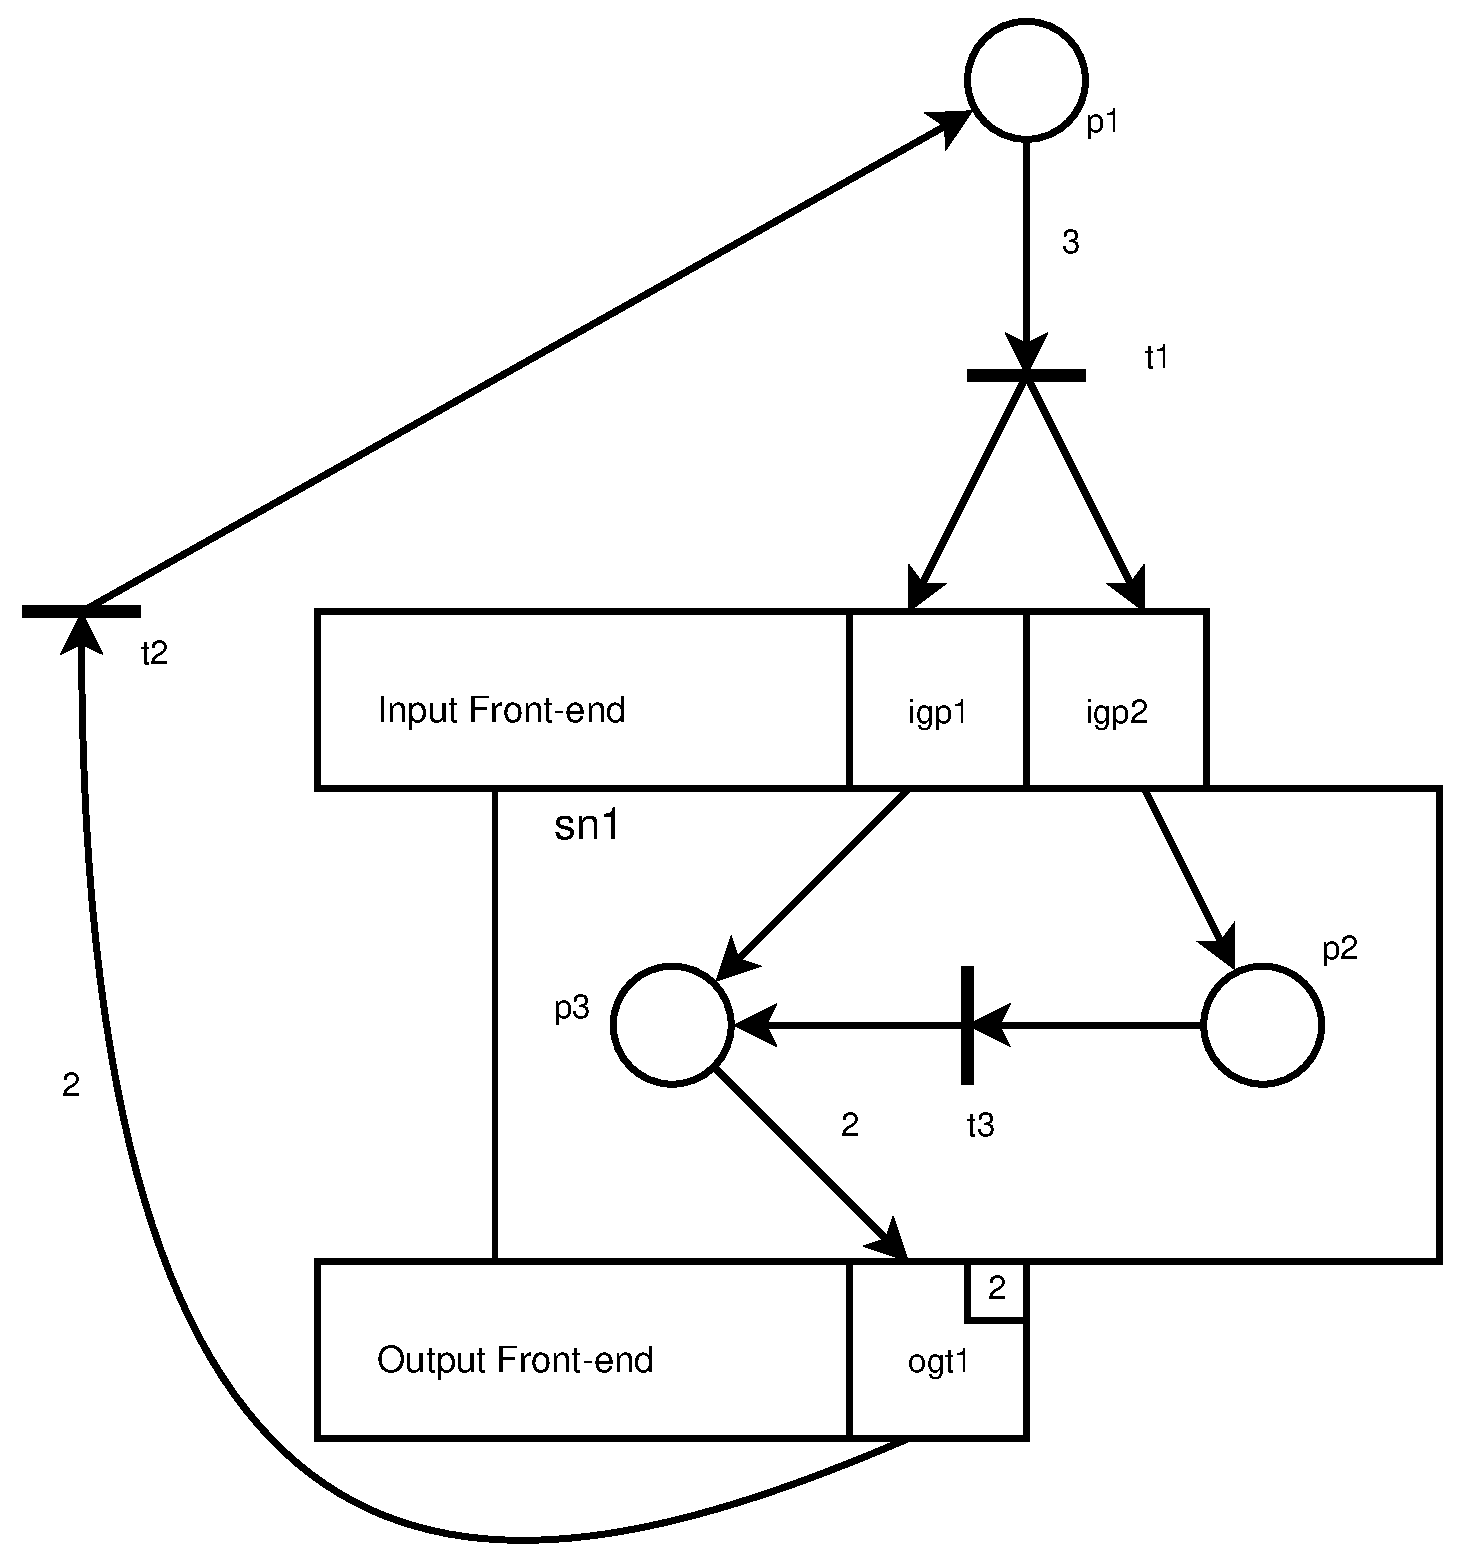
\includegraphics[width=0.60\textwidth]{Figures/PNML-SubredEjemplo1.eps}
\]

and its full PNML representation:

\begin{lstlisting}
<?xml version="1.0" encoding="utf-8"?>
<pnml>
  <net id="myNet" type="http://www.pnml.org/version-2009/grammar/ptnet">
    <name>
      <text> My new net </text>
    </name>
    <page id="page1">
      <subnet id="sn1">
        <interface id="sn1-interface">
        <gate id="igp1" action="input" type="place"/>
        <gate id="igp2" action="input" type="place"/>
        <gate id="ogt1" action="output" type="transition">
          <inscription>
          <text> 2 </text>
          </inscription>
        </gate>
        </interface>
        <content id="sn1-content">
        <place id="p2"/>
        <place id="p3"/>
        <transition id="t3"/>
        <arc id="a2" source="igp2" target="p2"/>
        <arc id="a3" source="igp1" target="p3"/>
        <arc id="a4" source="p3" target="ogt1">
          <inscription>
          <text> 2 </text>
          </inscription>
        </arc>
        <arc id="a5" source="t3" target="p3"/>
        <arc id="a6" source="p2" target="t3"/>
        </content>
      </subnet>
      <place id="p1"/>
      <transition id="t1"/>
      <transition id="t2"/>
      <arc id="a1" source="p1" target="t1">
        <inscription>
        <text> 3 </text>
        </inscription>
      </arc>
      <arc id="a2" source="t1" target="igp2"/>
      <arc id="a3" source="t1" target="igp1"/>
      <arc id="a4" source="ogt1" target="t2">
        <inscription>
        <text> 2 </text>
        </inscription>
      </arc>
      <arc id="a7" source="t2" target="p1"/>
    </page>
  </net>
</pnml>
\end{lstlisting}

The first option is to sign the whole net. In XPath, the expression to represent
the entire document is:

\begin{lstlisting}[basicstyle=\ttfamily\small]
/ 
\end{lstlisting}

If we apply XMLSignature with this XPath expression, the result is

\begin{lstlisting}[basicstyle=\ttfamily\tiny]
<?xml version="1.0" encoding="UTF-8"?>
<pnml>
  <net id="myNet" type="http://www.pnml.org/version-2009/grammar/ptnet">
    <name>
      <text> My new net </text>
    </name>
    <page id="page1">
      <subnet id="sn1">
        <interface id="sn1-interface">
          <gate action="input" id="igp1" type="place"/>
          <gate action="input" id="igp2" type="place"/>
          <gate action="output" id="ogt1" type="transition">
            <inscription>
              <text> 2 </text>
            </inscription>
          </gate>
        </interface>
        <content id="sn1-content">
          <place id="p2"/>
          <place id="p3"/>
          <transition id="t3"/>
          <arc id="a2" source="igp2" target="p2"/>
          <arc id="a3" source="igp1" target="p3"/>
          <arc id="a4" source="p3" target="ogt1">
            <inscription>
              <text> 2 </text>
            </inscription>
          </arc>
          <arc id="a5" source="t3" target="p3"/>
          <arc id="a6" source="p2" target="t3"/>
        </content>
      </subnet>
      <place id="p1"/>
      <transition id="t1"/>
      <transition id="t2"/>
      <arc id="a1" source="p1" target="t1">
        <inscription>
          <text> 3 </text>
        </inscription>
      </arc>
      <arc id="a2" source="t1" target="igp2"/>
      <arc id="a3" source="t1" target="igp1"/>
      <arc id="a4" source="ogt1" target="t2">
        <inscription>
          <text> 2 </text>
        </inscription>
      </arc>
      <arc id="a7" source="t2" target="p1"/>
    </page>
  </net>
  <ds:Signature xmlns:ds="http://www.w3.org/2000/09/xmldsig#">
    <ds:SignedInfo>
      <ds:CanonicalizationMethod Algorithm="http://www.w3.org/TR/2001/REC-xml-c14n-20010315"/>
      <ds:SignatureMethod Algorithm="http://www.w3.org/2000/09/xmldsig#rsa-sha1"/>
      <ds:Reference URI="">
        <ds:Transforms>
          <ds:Transform Algorithm="http://www.w3.org/2000/09/xmldsig#enveloped-signature"/>
          <ds:Transform Algorithm="http://www.w3.org/TR/2001/REC-xml-c14n-20010315#WithComments"/>
          <ds:Transform Algorithm="http://www.w3.org/2002/06/xmldsig-filter2">
            <dsig-xpath:XPath xmlns:dsig-xpath="http://www.w3.org/2002/06/xmldsig-filter2" Filter="union">
              /
            </dsig-xpath:XPath>
          </ds:Transform>
        </ds:Transforms>
        <ds:DigestMethod Algorithm="http://www.w3.org/2000/09/xmldsig#sha1"/>
        <ds:DigestValue>LIMSPHwtGpK3hlDEdfaAv7D39KU=</ds:DigestValue>
      </ds:Reference>
    </ds:SignedInfo>
    <ds:SignatureValue>
      W3C5nlPSYcR2qvx2bOwpGy8CGMu0vWPTZCIQVkYuGUA52lRmtyFRInlRm0G+d+eqQHBwtvMophte
      HWPsPiOl+Bwc/C3HTHj2XBc9P1bcFUtVM91rLhLZhI/ZAl9t6VfLoQ+Cduu8sQJh6qiH24CiYGjc
      FaOlQbQ0sYBvGXoBhEk=
    </ds:SignatureValue>
    <ds:KeyInfo>
      <ds:X509Data>
        <ds:X509Certificate>
          MIICgTCCAeqgAwIBAgIETfh4CTANBgkqhkiG9w0BAQUFADCBhDELMAkGA1UEBhMCRVMxETAPBgNV
          BAgTCExBIFJJT0pBMREwDwYDVQQHDAhMT0dST8KlTzEgMB4GA1UEChMXVU5JVkVSU0lEQUQgREUg
          TEEgUklPSkExDDAKBgNVBAsTA1BGQzEfMB0GA1UEAwwWScKlSUdPIExFw6BOIFNBTUFOSUVHTzAe
          Fw0xMTA2MTUwOTE0NDlaFw0xMTA5MTMwOTE0NDlaMIGEMQswCQYDVQQGEwJFUzERMA8GA1UECBMI
          TEEgUklPSkExETAPBgNVBAcMCExPR1JPwqVPMSAwHgYDVQQKExdVTklWRVJTSURBRCBERSBMQSBS
          SU9KQTEMMAoGA1UECxMDUEZDMR8wHQYDVQQDDBZJwqVJR08gTEXDoE4gU0FNQU5JRUdPMIGfMA0G
          CSqGSIb3DQEBAQUAA4GNADCBiQKBgQChePFNVCIfphFlyXQ9BysiR5BfXIuv3AnAK80Fuw4tTFwC
          nVUjJeGnkUYQO32oUu+fEBK8WsEqjeH8A7zrHTRQjfYZWyuGWrM8gJXOa/P0MROPm/c/H8b5a6Nx
          1/+zLwR0tYkqLI2xqDOFII2RwK5L2yGeV4T4y8i3h1U0OFTSEwIDAQABMA0GCSqGSIb3DQEBBQUA
          A4GBAIDOvAAdOCaTpy+83bGB2KmngMJrNxxWDpAi5LGFrN8iCShmbTpIeIbYBUAaBpZtdhOnhq4n
          wD5QOENSFipQcdH5GEpPM9Rquy6xMwfda9EU5UfOSEmbk4fK2vaIOVjynpQsJ9P99enO2smQlyvw
          /hBa7Xacz6qDut8ghUeuV5Js
        </ds:X509Certificate>
      </ds:X509Data>
      <ds:KeyValue>
        <ds:RSAKeyValue>
          <ds:Modulus>
            oXjxTVQiH6YRZcl0PQcrIkeQX1yLr9wJwCvNBbsOLUxcAp1VIyXhp5FGEDt9qFLvnxASvFrBKo3h
            /AO86x00UI32GVsrhlqzPICVzmvz9DETj5v3Px/G+Wujcdf/sy8EdLWJKiyNsagzhSCNkcCuS9sh
            nleE+MvIt4dVNDhU0hM=
          </ds:Modulus>
          <ds:Exponent>AQAB</ds:Exponent>
        </ds:RSAKeyValue>
      </ds:KeyValue>
    </ds:KeyInfo>
  </ds:Signature>
</pnml>
\end{lstlisting}

In the generated \texttt{<Signature>} a XMLSignature XPath Filter tag has
appeared as a new \texttt{<Transform>}

\begin{lstlisting} 
<ds:Transform Algorithm="http://www.w3.org/2002/06/xmldsig-filter2">
  <dsig-xpath:XPath
      xmlns:dsig-xpath="http://www.w3.org/2002/06/xmldsig-filter2"
      Filter="union">
    /
  </dsig-xpath:XPath>
</ds:Transform>
\end{lstlisting}

It is easy to see the behaviour of this element: the union of "/" XPath expression,
that is to say, the union of the entire document.

The set of nodes returned by this expression is

\begin{lstlisting}
<pnml>
  <net id="myNet" type="http://www.pnml.org/version-2009/grammar/ptnet">
    <name>
      <text> My new net </text>
    </name>
    <page id="page1">
      <subnet id="sn1">
        <interface id="sn1-interface">
        <gate action="input" id="igp1" type="place"></gate>
        <gate action="input" id="igp2" type="place"></gate>
        <gate action="output" id="ogt1" type="transition">
          <inscription>
          <text> 2 </text>
          </inscription>
        </gate>
        </interface>
        <content id="sn1-content">
        <place id="p2"></place>
        <place id="p3"></place>
        <transition id="t3"></transition>
        <arc id="a2" source="igp2" target="p2"></arc>
        <arc id="a3" source="igp1" target="p3"></arc>
        <arc id="a4" source="p3" target="ogt1">
          <inscription>
          <text> 2 </text>
          </inscription>
        </arc>
        <arc id="a5" source="t3" target="p3"></arc>
        <arc id="a6" source="p2" target="t3"></arc>
        </content>
      </subnet>
      <place id="p1"></place>
      <transition id="t1"></transition>
      <transition id="t2"></transition>
      <arc id="a1" source="p1" target="t1">
        <inscription>
        <text> 3 </text>
        </inscription>
      </arc>
      <arc id="a2" source="t1" target="igp2"></arc>
      <arc id="a3" source="t1" target="igp1"></arc>
      <arc id="a4" source="ogt1" target="t2">
        <inscription>
        <text> 2 </text>
        </inscription>
      </arc>
      <arc id="a7" source="t2" target="p1"></arc>
    </page>
  </net>
</pnml> 
\end{lstlisting}

It is the full document (without the first row xml definition) node set.

Other important configuration in this work is the signing of a concrete subnet. In this case, it is a little different as in XMLEncryption. Remember that in XMLEncription, if I want to mask a subnet I don't process the \texttt{<subnet>} tag
but the \texttt{subnet/content} this is because the interface has to be visible.
But in a signature I want to sign the complete subnet, including the interface.
Suppose that this subnet has \texttt{id="sn1"}. The XPath expression that
represents it is

\begin{lstlisting}[basicstyle=\ttfamily\small]
/net/page/subnet[@id="sn1"] 
\end{lstlisting}

The node set in this case is

\begin{lstlisting}[basicstyle=\ttfamily\tiny]
<subnet id="sn1">
  <interface id="sn1-interface">
    <gate action="input" id="igp1" type="place"/>
    <gate action="input" id="igp2" type="place"/>
    <gate action="output" id="ogt1" type="transition">
      <inscription>
        <text> 2 </text>
      </inscription>
    </gate>
  </interface>
  <content id="sn1-content">
    <place id="p2"/>
    <place id="p3"/>
    <transition id="t3"/>
    <arc id="a2" source="igp2" target="p2"/>
    <arc id="a3" source="igp1" target="p3"/>
    <arc id="a4" source="p3" target="ogt1">
      <inscription>
        <text> 2 </text>
      </inscription>
    </arc>
    <arc id="a5" source="t3" target="p3"/>
    <arc id="a6" source="p2" target="t3"/>
  </content>
</subnet>
\end{lstlisting}

and the signature result is

\begin{lstlisting}[basicstyle=\ttfamily\tiny]
<?xml version="1.0" encoding="UTF-8"?>
<pnml>
  <net id="myNet" type="http://www.pnml.org/version-2009/grammar/ptnet">
    <name>
      <text> My new net </text>
    </name>
    <page id="page1">
      <subnet id="sn1">
        <interface id="sn1-interface">
          <gate action="input" id="igp1" type="place"/>
          <gate action="input" id="igp2" type="place"/>
          <gate action="output" id="ogt1" type="transition">
            <inscription>
              <text> 2 </text>
            </inscription>
          </gate>
        </interface>
        <content id="sn1-content">
          <place id="p2"/>
          <place id="p3"/>
          <transition id="t3"/>
          <arc id="a2" source="igp2" target="p2"/>
          <arc id="a3" source="igp1" target="p3"/>
          <arc id="a4" source="p3" target="ogt1">
            <inscription>
              <text> 2 </text>
            </inscription>
          </arc>
          <arc id="a5" source="t3" target="p3"/>
          <arc id="a6" source="p2" target="t3"/>
        </content>
      </subnet>
      <place id="p1"/>
      <transition id="t1"/>
      <transition id="t2"/>
      <arc id="a1" source="p1" target="t1">
        <inscription>
          <text> 3 </text>
        </inscription>
      </arc>
      <arc id="a2" source="t1" target="igp2"/>
      <arc id="a3" source="t1" target="igp1"/>
      <arc id="a4" source="ogt1" target="t2">
        <inscription>
          <text> 2 </text>
        </inscription>
      </arc>
      <arc id="a7" source="t2" target="p1"/>
    </page>
  </net>
  <ds:Signature xmlns:ds="http://www.w3.org/2000/09/xmldsig#">
    <ds:SignedInfo>
      <ds:CanonicalizationMethod Algorithm="http://www.w3.org/TR/2001/REC-xml-c14n-20010315"/>
      <ds:SignatureMethod Algorithm="http://www.w3.org/2000/09/xmldsig#rsa-sha1"/>
      <ds:Reference URI="">
        <ds:Transforms>
          <ds:Transform Algorithm="http://www.w3.org/2000/09/xmldsig#enveloped-signature"/>
          <ds:Transform Algorithm="http://www.w3.org/TR/2001/REC-xml-c14n-20010315#WithComments"/>
          <ds:Transform Algorithm="http://www.w3.org/2002/06/xmldsig-filter2">
            <dsig-xpath:XPath xmlns:dsig-xpath="http://www.w3.org/2002/06/xmldsig-filter2" Filter="intersect">
              /pnml/net/page/subnet[@id="sn1"]
            </dsig-xpath:XPath>
          </ds:Transform>
        </ds:Transforms>
        <ds:DigestMethod Algorithm="http://www.w3.org/2000/09/xmldsig#sha1"/>
        <ds:DigestValue>prCzhLgTCZ1ck6MjQnFy6cASCZw=</ds:DigestValue>
      </ds:Reference>
    </ds:SignedInfo>
    <ds:SignatureValue>
      QoO7mQmGBFTg2UxgiZnzlsnKi8V477JC0v12JPItL53zIOCpjhOwLoyxENl6v8lCLoJ9WwFHlBKk
      r3GdqrgZimNXMUjwR4zkd9FVNcIrn85DuRjHA/zDwSuPMq9w0N5A07c0xJ24uvn9+zpbQxfblYTb
      kiy08+S0pqczU/bv5+g=
    </ds:SignatureValue>
    <ds:KeyInfo>
      <ds:X509Data>
        <ds:X509Certificate>
          MIICgTCCAeqgAwIBAgIETfh4CTANBgkqhkiG9w0BAQUFADCBhDELMAkGA1UEBhMCRVMxETAPBgNV
          BAgTCExBIFJJT0pBMREwDwYDVQQHDAhMT0dST8KlTzEgMB4GA1UEChMXVU5JVkVSU0lEQUQgREUg
          TEEgUklPSkExDDAKBgNVBAsTA1BGQzEfMB0GA1UEAwwWScKlSUdPIExFw6BOIFNBTUFOSUVHTzAe
          Fw0xMTA2MTUwOTE0NDlaFw0xMTA5MTMwOTE0NDlaMIGEMQswCQYDVQQGEwJFUzERMA8GA1UECBMI
          TEEgUklPSkExETAPBgNVBAcMCExPR1JPwqVPMSAwHgYDVQQKExdVTklWRVJTSURBRCBERSBMQSBS
          SU9KQTEMMAoGA1UECxMDUEZDMR8wHQYDVQQDDBZJwqVJR08gTEXDoE4gU0FNQU5JRUdPMIGfMA0G
          CSqGSIb3DQEBAQUAA4GNADCBiQKBgQChePFNVCIfphFlyXQ9BysiR5BfXIuv3AnAK80Fuw4tTFwC
          nVUjJeGnkUYQO32oUu+fEBK8WsEqjeH8A7zrHTRQjfYZWyuGWrM8gJXOa/P0MROPm/c/H8b5a6Nx
          1/+zLwR0tYkqLI2xqDOFII2RwK5L2yGeV4T4y8i3h1U0OFTSEwIDAQABMA0GCSqGSIb3DQEBBQUA
          A4GBAIDOvAAdOCaTpy+83bGB2KmngMJrNxxWDpAi5LGFrN8iCShmbTpIeIbYBUAaBpZtdhOnhq4n
          wD5QOENSFipQcdH5GEpPM9Rquy6xMwfda9EU5UfOSEmbk4fK2vaIOVjynpQsJ9P99enO2smQlyvw
          /hBa7Xacz6qDut8ghUeuV5Js
        </ds:X509Certificate>
      </ds:X509Data>
      <ds:KeyValue>
        <ds:RSAKeyValue>
          <ds:Modulus>
            oXjxTVQiH6YRZcl0PQcrIkeQX1yLr9wJwCvNBbsOLUxcAp1VIyXhp5FGEDt9qFLvnxASvFrBKo3h
            /AO86x00UI32GVsrhlqzPICVzmvz9DETj5v3Px/G+Wujcdf/sy8EdLWJKiyNsagzhSCNkcCuS9sh
            nleE+MvIt4dVNDhU0hM=
          </ds:Modulus>
          <ds:Exponent>AQAB</ds:Exponent>
        </ds:RSAKeyValue>
      </ds:KeyValue>
    </ds:KeyInfo>
  </ds:Signature>
</pnml>
\end{lstlisting}

In this case, the Transform associated to the XPath expression is
\begin{lstlisting}
<ds:Transform Algorithm="http://www.w3.org/2002/06/xmldsig-filter2">
  <dsig-xpath:XPath
      xmlns:dsig-xpath="http://www.w3.org/2002/06/xmldsig-filter2"
      Filter="intersect">
    /pnml/net/page/subnet[@id="sn1"]
  </dsig-xpath:XPath>
</ds:Transform>
\end{lstlisting}

As we can see, the resultant node set is the intersection of the entire document
and the nodes returned by \texttt{/pnml/net/page/subnet[@id="sn1"]}, that
is, the nodes returned by \texttt{/pnml/net/page/subnet[@id="sn1"]}. 






\section{Examples}

\subsection{Signing all the subnets of a Petri net}

Other important configuration is to sign all the subnets defined in
a PNML file. Let's take the example Petri net of the section \ref{Example several subnets}. The goal is to sign all the subnets...
//TODO

\subsection{Signing several different subnets}

In this part a configuration is to sign several subnets (but not all) defined in
a PNML file is explained. Taking the example of the section \ref{Example several subnets} 

//TODO

\subsection{Signing hidden subnets}

In this last section, I am going to explain the full process of securizing
a Petri net, using both XMLEncryption and XMLSignature. If I want to take
advantage of this two technologies 
\section{Conclusions}


